\section{Introduction}\label{sec:intro}

Getting a quicker validation of the proposed product is crucial in the era of fierce competition and faster obsolescence. Digital product development, which includes, modeling by CAD and analysis by CAE plays a crucial role in quicker ``Time to market''.  For sheet-metal/plastic products (generically classified as `thin-walled'),  a quicker and fairly accurate CAE analysis is possible by idealizing their solid models to the equivalent surface representation called ``Midsurface''. Midsurface can be envisaged as a surface lying midway of a thin-walled solid, and mimicking it.   In CAE analysis, instead of using expensive 3D elements, 2D elements are used on the midsurface for fairly accurate results in far lesser computations/time. Because of this  advantage, midsurface is widely used and is available in many commercial CAD-CAE packages.  Even in this age of scalable and near-infinite computing power, it is still desirable to have  a robust and well-connected midsurface, so as to run more design iterations quickly.  \footnote{By ``robust'', it is meant that any small change in the input model should not have dramatic effect on the output midsurface and by ``well-connected'', it is meant that the midsurface should not have any gaps or overlaps and it should mimic the input correctly, especially at the connections.}

\begin{figure}[!htp]
\centering
\includegraphics[width=0.6\linewidth]{..//Common/images/MidsurfaceErrorsMscApex}
\caption{Midsurface Errors (Source: \cite{MScApex})}
\label{fig:midsurfaceerrors}
\end{figure}

In spite of its demand and popularity, the existing techniques for computing the midsurface fail to compute a well-connected midsurface, especially for non-trivial shapes \cite{ Robinson2006, Stolt2006a,Lockett2008, Woo2013,Automex}. Failures manifest in the form of gaps, missing patches, overlapping surfaces, not lying midway, not mimicking the input shape, etc. (Figure \ref{fig:midsurfaceerrors}). Correcting these errors is mostly a manual, tedious and highly time-consuming task, requiring hours to days. This correction time can be nearly equivalent to the time it can take to create the midsurface manually from scratch \cite{Stolt2006}. 

One of the major impediments in the development of the algorithm for automatic computation of the midsurface, is the lack of its precise definition \cite{Ramanathan2004}.  Expectations vary based on the application context (Figure \ref{fig:introduction:midsurfaceexptations}). For applications such as CAE, Figure ~\ref{fig:introduction:stairsfl} may be preferred over Figure ~\ref{fig:introduction:stairsmk} which is best suited for  shape matching/retrieval. Figure ~\ref{fig:introduction:stairsseparate} may be used where a disconnect needs to be highlighted. Figure ~\ref{fig:introduction:stairsmk} is considered as the choice of midsurface for this work. The variations shown in Figure \ref{fig:introduction:midsurfaceexptations} pertain to geometries computed  at the interfaces, and the proposed method can cater to them too with additional rules (for future scope). For specific applications such as CAE, additional rules, such as use of symmetry, specification of continuity between patches, etc. can also be incorporated to further customize the midsurface. 

\def \myfigstairspcolumnwidth{0.22}

\begin{figure}[h!]
\centering     %%% not \center
\subfloat[Model]{\label{fig:introduction:stairsmodel}\includegraphics[width=\myfigstairspcolumnwidth\linewidth]{../Common/images/Stairs_part.pdf}} \quad
\subfloat[Gradual]{\label{fig:introduction:stairsfl}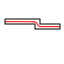
\includegraphics[width=\myfigstairspcolumnwidth\linewidth]{../Common/images/Stairs_follows.pdf}}  \quad
\subfloat[Mimicking]{\label{fig:introduction:stairsmk}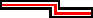
\includegraphics[width=\myfigstairspcolumnwidth\linewidth]{../Common/images/Stairs_mimic.pdf}}   \quad
\subfloat[Disjoint]{\label{fig:introduction:stairsseparate}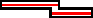
\includegraphics[width=\myfigstairspcolumnwidth\linewidth]{../Common/images/Stairs_separate.pdf}}
\caption{Expectations vary with regards to desired Midsurface}
\label{fig:introduction:midsurfaceexptations}
\end{figure}


Motivation of this work  is to address midsurface problems by leveraging feature-based simplification, abstraction and decomposition in a generic manner. Advantages can be seen in the form of range of shapes handled as well as in the minimization of failures.


%\begin{minipage}[h]{0.98\linewidth} 
%\begin{minipage}[h]{0.34\linewidth} 
%		\centering
%		\includegraphics[width=\linewidth]{..//Common/images/MidsurfaceErrorsMscApex}
%		\captionof{figure}{Midsurface Errors (Source: \cite{MScApex})}
%		\label{fig:midsurfaceerrors}
%\end{minipage}
%\hfill
%\begin{minipage}[h]{0.64\linewidth} 
%
%
%In spite of its demand and popularity, the existing techniques of computing the midsurface fail to compute a well-connected midsurface, especially for non-trivial shapes (\cite{ Robinson2006, Stolt2006a,Lockett2008, Woo2013,Automex}). Failures manifest in the form of gaps, missing patches, overlapping surfaces, not lying midway, not mimicking the input shape, etc. (Figure \ref{fig:midsurfaceerrors}). Correcting these errors is mostly a manual, tedious and highly time-consuming task, requiring hours to days. This correction time can be nearly equivalent to the time it can take to create the midsurface manually from scratch (\cite{Stolt2006}). 
%
%\end{minipage}
%\end{minipage}
%\end{figure}





